The purpose of this chapter is to provide a quantifiable assessment of the persistent radio wave energy in the near-Earth space environment due to lightning-generated Whistlers.



\section{Overview of Previous Work}

\section{Methodology}

\begin{figure}[ht]
\begin{center}
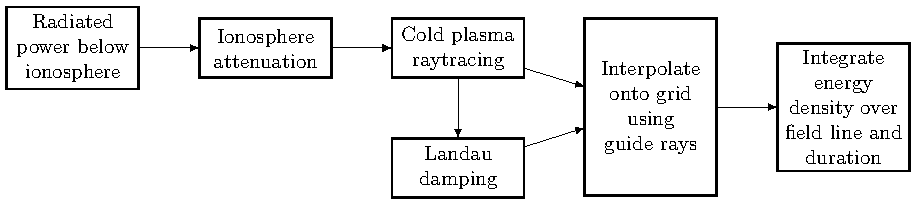
\includegraphics{figures/lightning_power_block_diagram.pdf}



\caption{Block diagram}
\label{fig:power_blockdiagram}
\end{center}
\end{figure}

\subsection{Gridding and Interpolation}

\begin{figure}[ht]
\begin{center}
\includegraphics[draft]{figures/interpolation_scheme.pdf}
\caption{Interpolation scheme}
\label{fig:interpolation_scheme}
\end{center}
\end{figure}

\subsection{Persistent Energy from a Single Flash}

\begin{figure}[ht]
\begin{center}
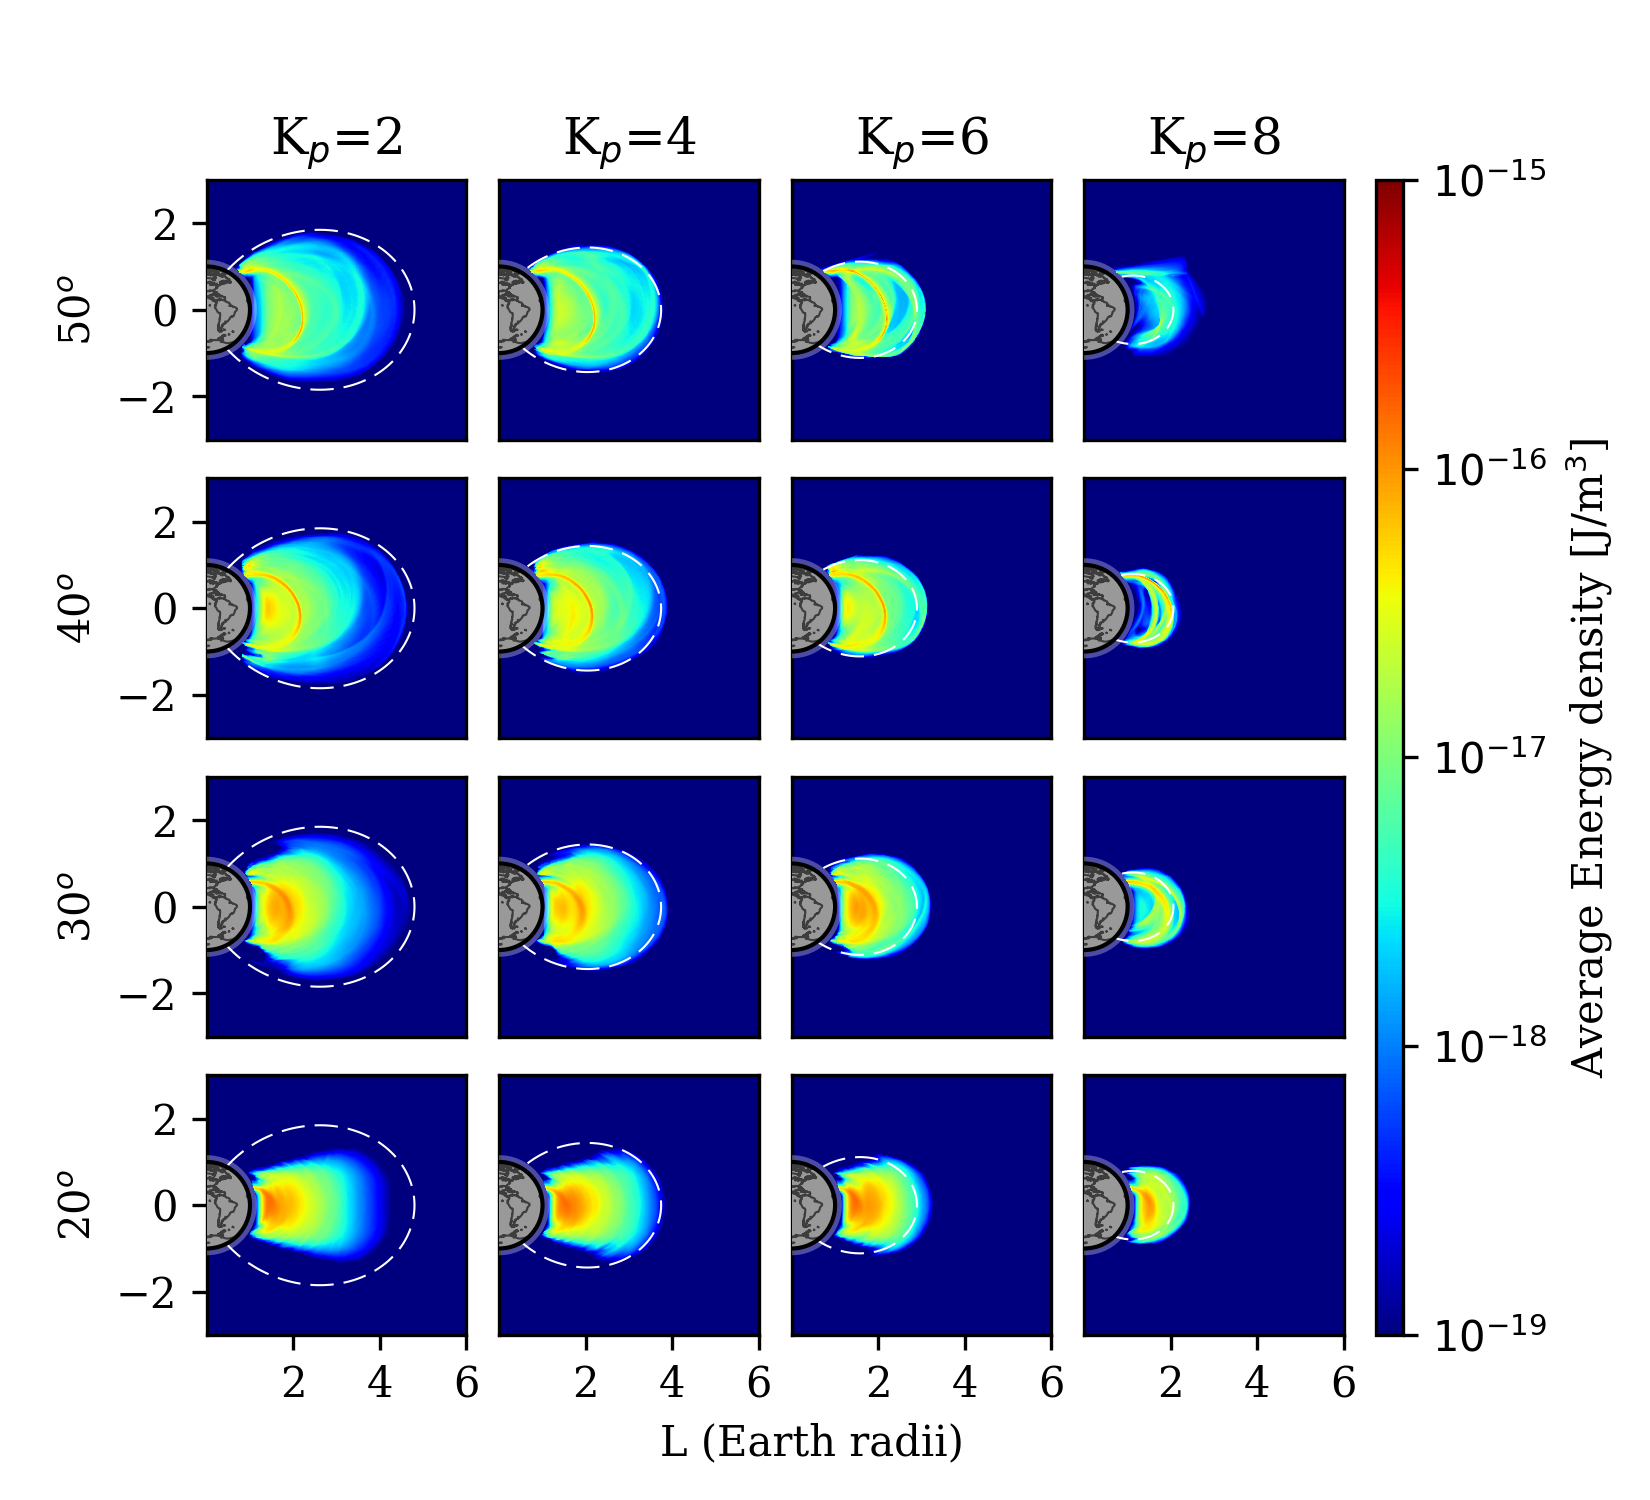
\includegraphics[draft]{figures/energy_from_single_flash_meridonal_plane.pdf}
\caption{Block diagram}
\label{fig:energy_from_single_flash}
\end{center}
\end{figure}

% you'll want to put a figure showing the volume averaging too...

\begin{figure}[ht]
\begin{center}
\includegraphics[draft]{figures/energy_stencils.pdf}
\caption{Block diagram}
\label{fig:energy_stencils}
\end{center}
\end{figure}

\subsection{Global Energy Density}